\chapter{Background}
\label{chap:background}
Il presente capitolo introduce il contesto tecnico e infrastrutturale all'interno del quale si colloca il lavoro di tesi. 
In particolare, viene descritta l'architettura legacy del servizio di misurazione della latenza attualmente in produzione, sviluppato per supportare le esigenze operative di \emph{FlashStart Cloud}.
La comprensione approfondita di tale architettura, delle sue componenti e delle interazioni tra di esse costituisce un prerequisito indispensabile per individuare i limiti del sistema esistente e per motivare le scelte progettuali presentate nei capitoli successivi.

Di seguito viene descritta nel dettaglio l'architettura a tre componenti --- Upstream Orchestrator, Downstream e route PHP --- che costituisce il punto di partenza dell'analisi condotta in questo lavoro.

Il servizio di misurazione della latenza (di seguito \emph{latency service}) adotta un'architettura distribuita a tre componenti disaccoppiati, ciascuno responsabile di una fase distinta del processo di raccolta, aggregazione ed esposizione dei dati.
Le componenti comunicano tra loro in sequenza tramite chiamate \ac{HTTP}, secondo un modello \emph{orchestrator--worker} ricorrente nei sistemi progettati per il monitoraggio distribuito di infrastrutture di rete su larga scala.
La Figura~\ref{fig:legacy-architecture} illustra schematicamente il flusso di comunicazione tra le tre componenti; di seguito ciascuna di esse viene descritta in dettaglio.

\section{Upstream Orchestrator}
\label{section:upstream-orchestrator}

L'\emph{Upstream Orchestrator} rappresenta il componente centrale del sistema ed è localizzato all'interno del server principale dell'infrastruttura. Le sue responsabilità principali sono le seguenti:

\begin{itemize}
    \item \emph{Discovery dei server attivi}: recupera dinamicamente la lista dei server della rete da interrogare ai fini della misurazione della latenza, garantendo che solo i nodi effettivamente operativi vengano coinvolti nel processo di raccolta;
    \item \emph{Distribuzione delle richieste}: inoltra, tramite chiamate \ac{HTTP}, le richieste di misurazione verso ciascun nodo Downstream individuato nella fase precedente;
    \item \emph{Aggregazione dei risultati}: raccoglie le risposte provenienti dai singoli nodi Downstream, effettuando l'unione dei dati parziali in un'unica struttura coerente;
    \item \emph{Riordinamento}: applica un criterio di ordinamento ai risultati aggregati per valore di latenza crescente, in modo da restituire un output immediatamente consultabile dal componente che effettua la richiesta finale.
\end{itemize}

Essendo un componente unico e centralizzato, l'Upstream Orchestrator costituisce, come si vedrà, anche un potenziale un collo di bottiglia in termini di prestazioni al crescere del numero di nodi da interrogare.

\subsection{Struttura}
Internamente, l'Upstream Orchestrator non è implementato come un blocco monolitico, bensì risulta suddiviso in due sotto-componenti distinte, realizzate con tecnologie differenti e comunicanti tra loro tramite un meccanismo di invocazione locale.

\paragraph{Controller PHP.} Il primo elemento è un controller scritto in PHP, responsabile della gestione delle richieste in ingresso provenienti dai client (nello specifico, dalla route PHP di FlashStart Cloud descritta nella Sezione~\ref{section:route-php}). Il controller si occupa della validazione dei parametri ricevuti, dell'invocazione dello script Python descritto di seguito e della formattazione della risposta finale da restituire al chiamante.
In questo senso, il controller PHP svolge un ruolo di \emph{adapter}, disaccoppiando l'interfaccia esposta verso l'esterno dalla logica di orchestrazione vera e propria.

\paragraph{Script Python.} Il secondo elemento è uno script Python esterno, invocato dal controller PHP come processo separato, a cui è demandata la logica core dell'orchestrazione. In particolare, lo script è responsabile di eseguire le funzioni descritte in precedenza.

Al termine dell'elaborazione, lo script Python restituisce l'output al controller PHP, che ne cura la trasformazione nel formato di risposta atteso dal client.

\paragraph{Implicazioni architetturali.} Questa separazione tra controller PHP e script Python, per quanto funzionalmente sensata al momento della sua introduzione, comporta un'invocazione inter-processo ad ogni richiesta gestita dall'Orchestrator, con conseguente overhead in termini di latenza e complessità di gestione degli errori tra i due runtime.
Inoltre, la coesistenza di due linguaggi e stack tecnologici distinti all'interno dello stesso componente logico introduce un ulteriore fattore di complessità in termini di manutenibilità, testing e osservabilità del sistema, aspetti che verranno ripresi e discussi criticamente nei capitoli successivi.
\section{Downstream}
\label{section:downstream}

Il componente \emph{Downstream} è responsabile della misurazione puntuale del tempo di latenza tra il server su cui è in esecuzione e una macchina di destinazione specificata nella richiesta ricevuta dall'Upstream Orchestrator.
A differenza di quest'ultimo, il Downstream non è un componente unico, bensì viene replicato e distribuito su ciascuno dei DNS resolver appartenenti alla rete anycast del servizio.

Ogni istanza Downstream espone un singolo endpoint \ac{HTTP} che, ricevuta la richiesta dall'Orchestrator, esegue la misurazione e ne restituisce sincronamente il risultato.

\subsection{Struttura}
Analogamente all'Upstream Orchestrator, il Downstream è composto da un controller php e da un latency engine.

Il latency engine non è altro che uno script php esegue comandi shell di sistema \texttt{ping} o \texttt{ping6} gestendo l'output come stringa rigida.
Il parsing dell'output si basa su indici di riga fissi.

\lstinputlisting[float,language=c++,label={lst:ping-output}]{listings/Ping-example}

Il parser si aspetta come input una stringa con un formato specifico (\cref{lst:ping-output}) andando a leggere precisamente la settima riga ricavando il tempo medio di risposta attraverso semplici operazioni con le stringhe.
Questo metodo è altamente vulnerabile alle variazioni del sistema operativo target.

\section{La route \texttt{php}}
\label{section:route-php}

La terza componente del sistema è costituita da una \emph{route} implementata in PHP, utilizzata da FlashStart Cloud come punto di ingresso applicativo per invocare l'intero servizio ed esporne i risultati.
La route agisce come livello di presentazione: riceve le richieste provenienti dal client, le inoltra all'Upstream Orchestrator e restituisce al chiamante i dati di latenza aggregati e ordinati, in un formato adatto al consumo da parte dell'applicazione.

Questo script php riceve i dati dall'upstream orchestrator e inserisce informazioni aggiuntive riguardanti i singoli server interrogati.
Ha inoltre una funzione di filtraggio delle risposte duplicate, causate da un dispiegamento di più \ac{DNS} resolver in un unico server fisico.

\section{Flusso di comunicazione end-to-end}
\label{section:flusso-comunicazione}

Complessivamente, il flusso di una richiesta attraversa le tre componenti descritte secondo la seguente sequenza:

\begin{enumerate}
    \item Il client invoca la route PHP esposta da FlashStart Cloud;
    \item la route PHP inoltra la richiesta all'Upstream Orchestrator;
    \item l'Upstream Orchestrator recupera la lista dei server attivi e distribuisce, tramite chiamate HTTP, le richieste di misurazione ai relativi componenti Downstream dislocati sulla rete anycast;
    \item ciascun Downstream esegue la misurazione della latenza verso la macchina target e restituisce il risultato all'Orchestrator;
    \item l'Upstream Orchestrator aggrega e riordina i risultati ricevuti;
    \item il risultato finale viene restituito alla route PHP, che integra la risposta con informazioni aggiuntive e la espone al client.
\end{enumerate}

\begin{figure}
    \centering
    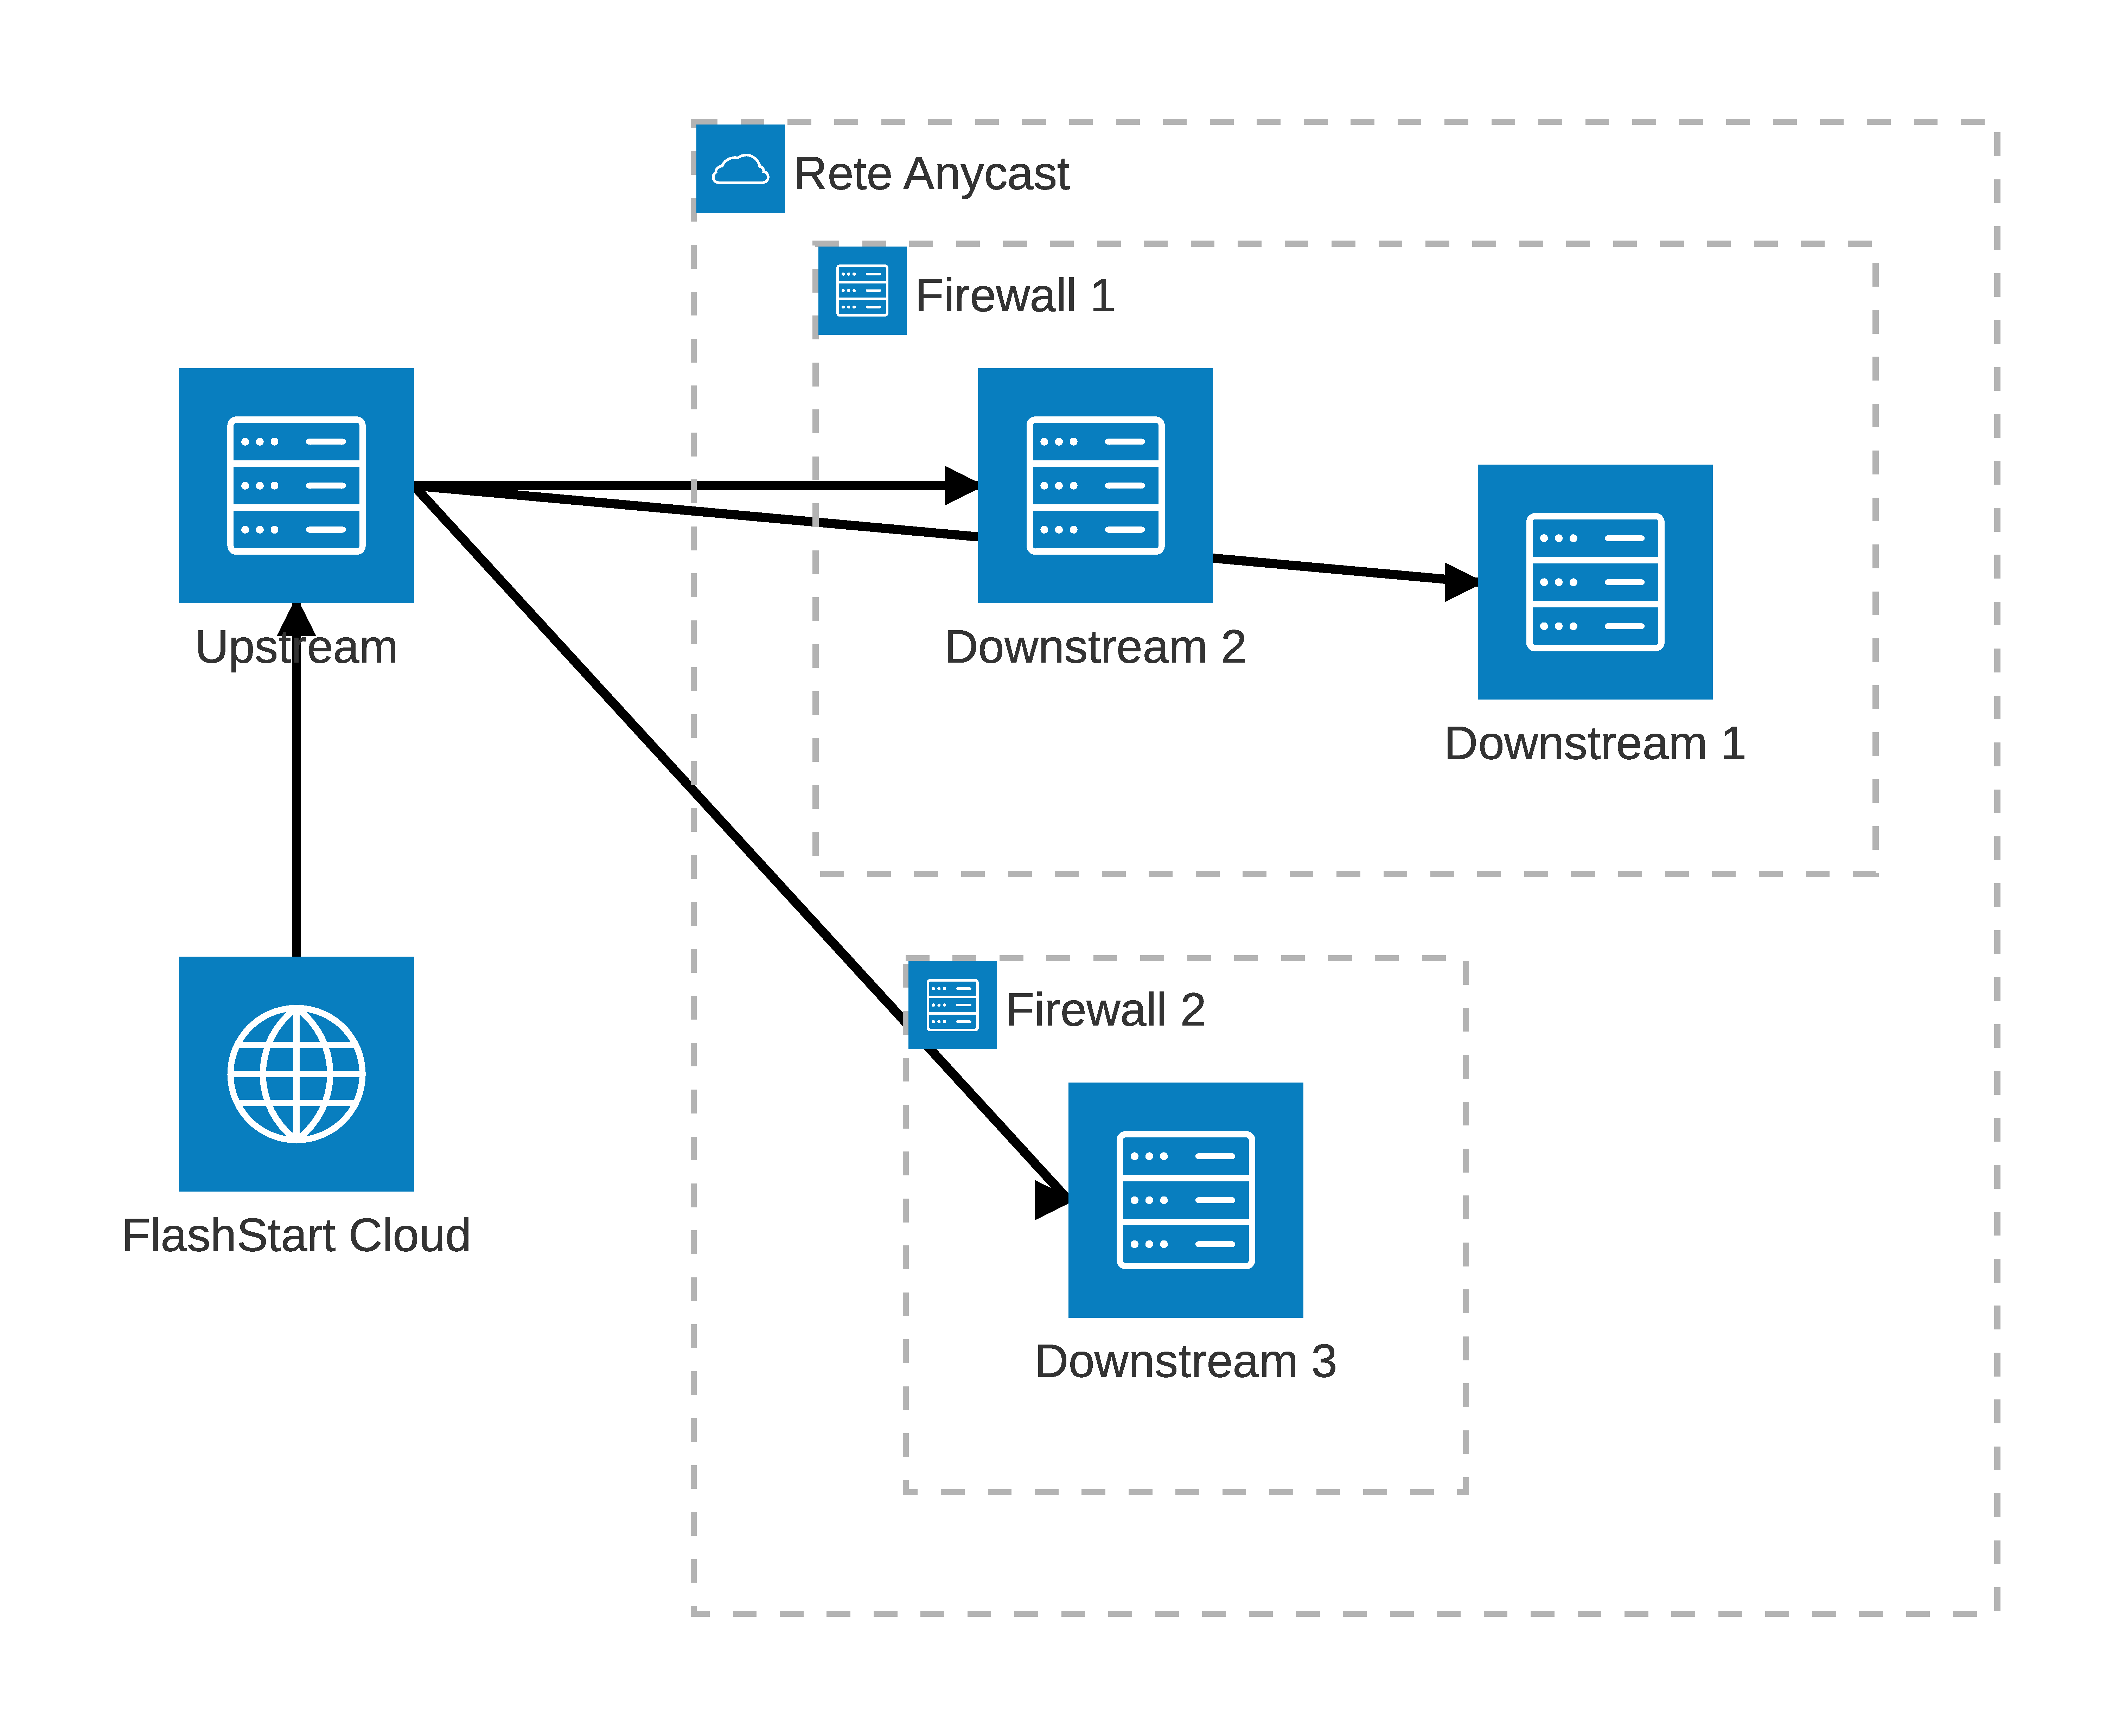
\includegraphics[width=.6\linewidth]{figures/legacy-architecture.pdf}
    \caption{Architettura del servizio legacy}
    \label{fig:legacy-architecture}
\end{figure}